\documentclass[10pt]{article}
\usepackage[style=authoryear, maxcitenames=2, mincitenames=1]{biblatex} % format citations auteurs
\usepackage{amsmath, amssymb} % better maths
\usepackage[draft]{graphicx} % Required for inserting images
\usepackage{geometry}
\usepackage{hyperref} %links
\usepackage{setspace} % spacing
\usepackage{dsfont} % pour le mathbb{1}
\usepackage{threeparttable} % comments table
\usepackage{longtable} % appendix
\usepackage{needspace} % longtable splits

\addbibresource{references.bib} % references
\geometry{a4paper, margin=2.5cm} % format
\renewcommand{\figurename}{\textsc{Figure}} % figure format
\renewcommand{\tablename}{\textsc{Table}} % table format
\renewcommand*{\nameyeardelim}{\addcomma\space} % name - comma - year format for citations

\begin{document}
\begin{setstretch}{1.1} % spacing
\setlength{\parindent}{0pt} % no indent


\section{Introduction}

\section{Data}


\subsection{Market data}

Binance, the world’s largest cryptocurrency exchange by trading volume, provides an exceptionally dense and \href{https://github.com/binance/binance-public-data}{well documented} \href{https://data.binance.vision}{public dataset} for all of its trading pairs. For spot pairs, it includes tick-by-tick trade history and candlestick data down to a 1-second resolution dating back to 2017. For our observation window, we store aggregated trades (3.7B rows) and 1-second price data (231M rows) into a DuckDB database for Ethereum-Tether (ETHUSDT) and Bitcoin-Tether (BTCUSDT) pairs. Tether pairs selection is justified by the market capitalization of this stablecoin -- ranked third behind Bitcoin and Ethereum -- and the substantial historical data available for these pairs on Binance. \medskip
%DuckDB table BTCUSDT_aggTrades: 2,645,406,584 rows
% DuckDB table BTCUSDT_1s_control: 115,825,966 rows, same for ETHUSDT
% DuckDB table ETHUSDT_aggTrades: 1,054,372,816 rows

In theory, aggregated trade data allows us to reconstruct precise higher-level aggregations by grouping trades over intervals of duration $N$. The effectiveness of this approach however depends on raw trades feeds fidelity. In practice, a 100\% Pearson correlation and a zero median discrepancy between downloaded and reconstructed 1-second data confirm the reliability of this method. We hence trust it for later bin size reconstruction. \medskip

Unlike traditional financial markets where prices are centralized, the cryptocurrency system is characterized by its fragmentation across multiple exchanges of varying volumes, listing closely aligned prices that would otherwise offer arbitrage opportunities (\cite{Makarov2020} \cite{Crepelliere2023}). For cross-validation of our Binance dataset, we use Coinbase, the second-largest exchange by volume. Its \href{https://docs.cdp.coinbase.com/api-reference/advanced-trade-api/rest-api/public/get-public-product-candles}{API} provides 1-minute historical candlestick data, which we extract via iterated request for both USDT and USD pairs. Coinbase's USDT and USD candlesticks are seemingly interchangeables, as underlined by a ~100\% Pearson correlation and a median absolute price difference situated below 0.05\% (below 0.3\% at the 99th percentile). However, their trading activity differ significantly: USD volumes are 25 to 35 times higher than those of USDT. We therefore select the former for subsequent inter-exchange comparisons. \medskip

Binance-Coinbase comparison reveals a ~100\% Pearson correlation and a median price difference below 0.02\% for candlestick data. Fewer than 0.01\% of 1-minute bins closing prices exhibit a discrepancy greater than 1\%, emphasizing limited upfront inter-exchange arbitrage opportunities. Given that Binance's USDT pairs have 78 to 128 times the volume of Coinbase USD contracts, we retain the former as our default data source from now on, unless mentioned otherwise. Other major exchanges (\href{https://support.kraken.com/articles/360047543791-downloadable-historical-market-data-time-and-sales-}{Kraken}, \href{https://public.bybit.com}{ByBit}) were evaluated as alternative data sources, but either lacked directly comparable trading pairs or provided limited historical coverage.\medskip


\subsection{Market Events}

To provide context for our empirical analysis, we compile a timeline of significant events affecting Ethereum and Bitcoin markets in the period surrounding The Merge. For Ethereum, sources include \href{https://ethereum.org/ethereum-forks/}{Ethereum Project's forks timeline} that lists major milestones of the blockchain, \href{https://blog.ethereum.org}{Ethereum Foundation's blog} and \href{https://www.eth101.org/en/history}{EHT101's timeline} discussing exogenous events affecting the crypto environment during Ethereum's lifespan. CoinMarketCap's all-time Ethereum and Bitcoin plots listing news and milestones, Binance archived announcements for fees regime, as well as \href{https://www.strategy.com/ledger}{Strategy's} Bitcoin purchases were also used. Events span two main categories: Ethereum's protocol upgrades (e.g. the Merge), and global market shocks (e.g. regulatory changes). Across hundreds of events, those listed in appendix ~\ref{sec:appendixEvents} are the shortlisted ones explaining major events for these markets over our timeframe. For further financial context, we obtain 5-minute interval S\&P500 OHLC data from a \href{https://www.kaggle.com/datasets/salaheddineelkhirani/5-year-data-for-s-and-p-500-and-nasdaq-100/data}{Kaggle dataset} matching our observation period, and weekly risk-free rate from \href{https://mba.tuck.dartmouth.edu/pages/faculty/ken.french/data_library.html}{Kenneth R. French's website}. 


\section{Metrics}
We compute intraday metrics to measure both volatility and liquidity. For each pair, metrics are derived from aggregated trade data grouped at given intraday frequencies ranging from 10ms to 1-hour bins, subsequently aggregated at a daily level. Considering the size of our dataset, loading it all at once would overcome physical RAM limitations for metrics computation. We hence use a day-to-day data streaming approach in order to stay within our computational capacities bounds. This process is slower -- taking over an hour -- but allows us to save daily aggregated metrics based on various bin sizes. \medskip

For returns, we choose a close-to-close measure over an open-to-close alternative, as the latter sometimes doesn't account for price movements occurring between the close of one bin and the open of the next. \medskip

Intraday volatility is not directly observable; only prices sampled at a given frequency $\Delta \tau$ can be. For day $t$ divided into $M$ intervals $t=t_0<t_1<...<t_M$, let $r_{t_i}$ denote intraday logarithmic returns over the $i$-th interval. We consider several estimators for volatility. We first use the Realized Variance ($RV_t$, Eq.~\ref{eq:rv}) as a benchmark estimator of daily variance that converges toward integrated volatility in the absence of jumps, as $M \rightarrow \infty$. For a jump-robust alternative, we implement the Bipower Variation ($BV_t^{\left\{ 1,1 \right\}}$, Eq. Eq.~\ref{eq:bv}) introduced by \textcite{Barndorff2004}. Realized Semi-variance ($RS^+$, $RS^-$, Eq.~\ref{eq:rs}) captures variance asymmetry based on sign returns, and is computed in order to distinguish the respective contributions of upside and downside risk to total volatility (\cite{Barndorff2010}). Finally, in order to leverage full candlestick data rather than log-returns alone, we include the Garman-Klass estimator ($G\text{-}K_t$, Eq.~\ref{eq:gk}) as an efficient zero-drift variance proxy (\cite{Garman1980}), alongside the Rogers-Satchell alternative ($R\text{-}S_t$, Eq.~\ref{eq:rgs}) which provides an unbiased variance estimate in case of price trends (\cite{Rogers1991}).

\begin{align}
RV_t&=\sum\limits^M_{i=1}r^2_{t_i}\tag{1} \label{eq:rv}\\
BV_t^{\{ 1,1 \}}&=BV_T=\frac{\pi}{2}\sum\limits^M_{j=2}|r_{t_j}||r_{t_{j-1}}| \tag{2} \label{eq:bv}\\
RS_t^{+}&=\sum\limits^M_{i=1}r^2_{t_1}\mathds{1}_{rt_i\geq0}\quad\text{and}\quad RS_t^{-}=\sum\limits^M_{i=1}r^2_{t_1}\mathds{1}_{rt_i\leq0} \tag{3} \label{eq:rs}\\
G\text{-}K_t &= 0.5\left[ \ln\left(\frac{H_t}{L_t}\right)\right]^2 - (2\ln 2-1)\left[\ln\left(\frac{C_t}{O_T}\right)\right]^2\tag{4} \label{eq:gk}\\
R\text{-}S_t &= \ln\left(\frac{H_t}{C_t}\right)\ln\left(\frac{H_t}{O_t}\right)/\ln\left(\frac{L_t}{C_t}\right)\ln\left(\frac{L_t}{O_t}\right) \tag{5} \label{eq:rgs}
\end{align} \medskip

Where $O_t, H_t, L_t, C_t$ represent open, high, low and close values for day $t$, respectively. \medskip

For illiquidity measure, we rely on three different estimators. First, Amihud's illiquidity ratio (\cite{Amihud2002}) (Eq.~\ref{eq:Amihud}) is the standard reference, measuring illiquidity as a ratio of absolute percentage return to dollar volume over a given period. Its main appeal is its simplicity and availability, requiring only price and volume data. \textcite{Ranaldo2022} recently proposed an alternative version of this ratio: the Realized Amihud (Eq.~\ref{eq:Ramihud}), exploiting intraday returns rather than a single daily return, by aggregating absolute intraday log-returns before dividing by daily volume. This refinement captures intraday variation that the tradition ratio would otherwise average out. Finally, Kyle’s lambda (\cite{Kyle1985}) (Eq.~\ref{eq:Kyle}) offers an alternative price-impact measure derived from the linear relationship between trade-induced order flow and price change. Unlike the previous two illiquidity estimators, this metric can only be computed from the tick-level our dataset provides, as it requires trade-by-trade data in order to obtain signed volume. \medskip

\begin{align}
Amihud_t&=\frac{|R_t|}{V_t}\tag{6} \label{eq:Amihud}\\
RAmihud_t&=\frac{\sum\limits^M_{i=1}|r_{t_i}|}{V_t}\tag{7} \label{eq:RAmihud}\\
\Delta p_{t_i} &= \lambda_t \cdot x_{t_i} + \varepsilon_{t_i} \tag{8} \label{eq:Kyle}
\end{align}

where $R_t$ is daily return and $V_t$ is the daily dollar volume. \medskip

Signature plots (Fig.~\ref{fig:signaturePlot}) allow us to observe the evolution of our metrics as bin size increases from 10ms to 1h. Microstructure noise is noticeable at the 10ms and 100ms intervals for return-based volatility metrics, while Garman-Klass and Rogers-Satchell -- which rely on OHLC prices -- are less affected by sampling size at these frequencies. A convergence emerges from 1s onward, with all volatility metrics giving tight readings at the 5m interval. This suggests that at the 5-minute frequency, choice of estimator matters little as they yield comparable results for later analysis. This high correlation in between estimators is confirmed by our heatmap analysis (Figure~\ref{fig:AppendixHeatmap}). For sided metrics, realized semi-variance show no marked asymmetry, consistent with rather balanced sided price movements. We therefore select 5m as the default bin size for subsequent plots and analysis, in a trade off between granularity fine enough to capture true volatility, while remaining unaffected by microstructure noise. This follows \textcite{Andersen2001}(ref dans Haugom) who argues that for a liquid market, 5-min sampling interval is optimal. \textcite{Bandi2006}, \textcite{Andersen2007}, \textcite{Patton2011} and \textcite{Haugom2014} also chose 5-min as their optimal sampling frequency. For liquidity metrics, Amihud ratio is computed on a daily basis and Kyle's $\lambda$ is obtained through trade data: they remain unaffected by bin size. Only Realized Amihud shows a clear decreasing trend of illiquidity as bin size increases. Larger bin size means larger volume, hence reduced market impact of normal-sized orders on markets where daily volume is measured in billions. \medskip


\begin{figure}[!htbp]
\centering
\caption{Signature plot of realized volatility and liquidity estimators across sampling frequencies (10ms to 1h), ETHUSDT \textit{\&} BTCUSDT}
\vspace{8pt}
\label{fig:signaturePlot}
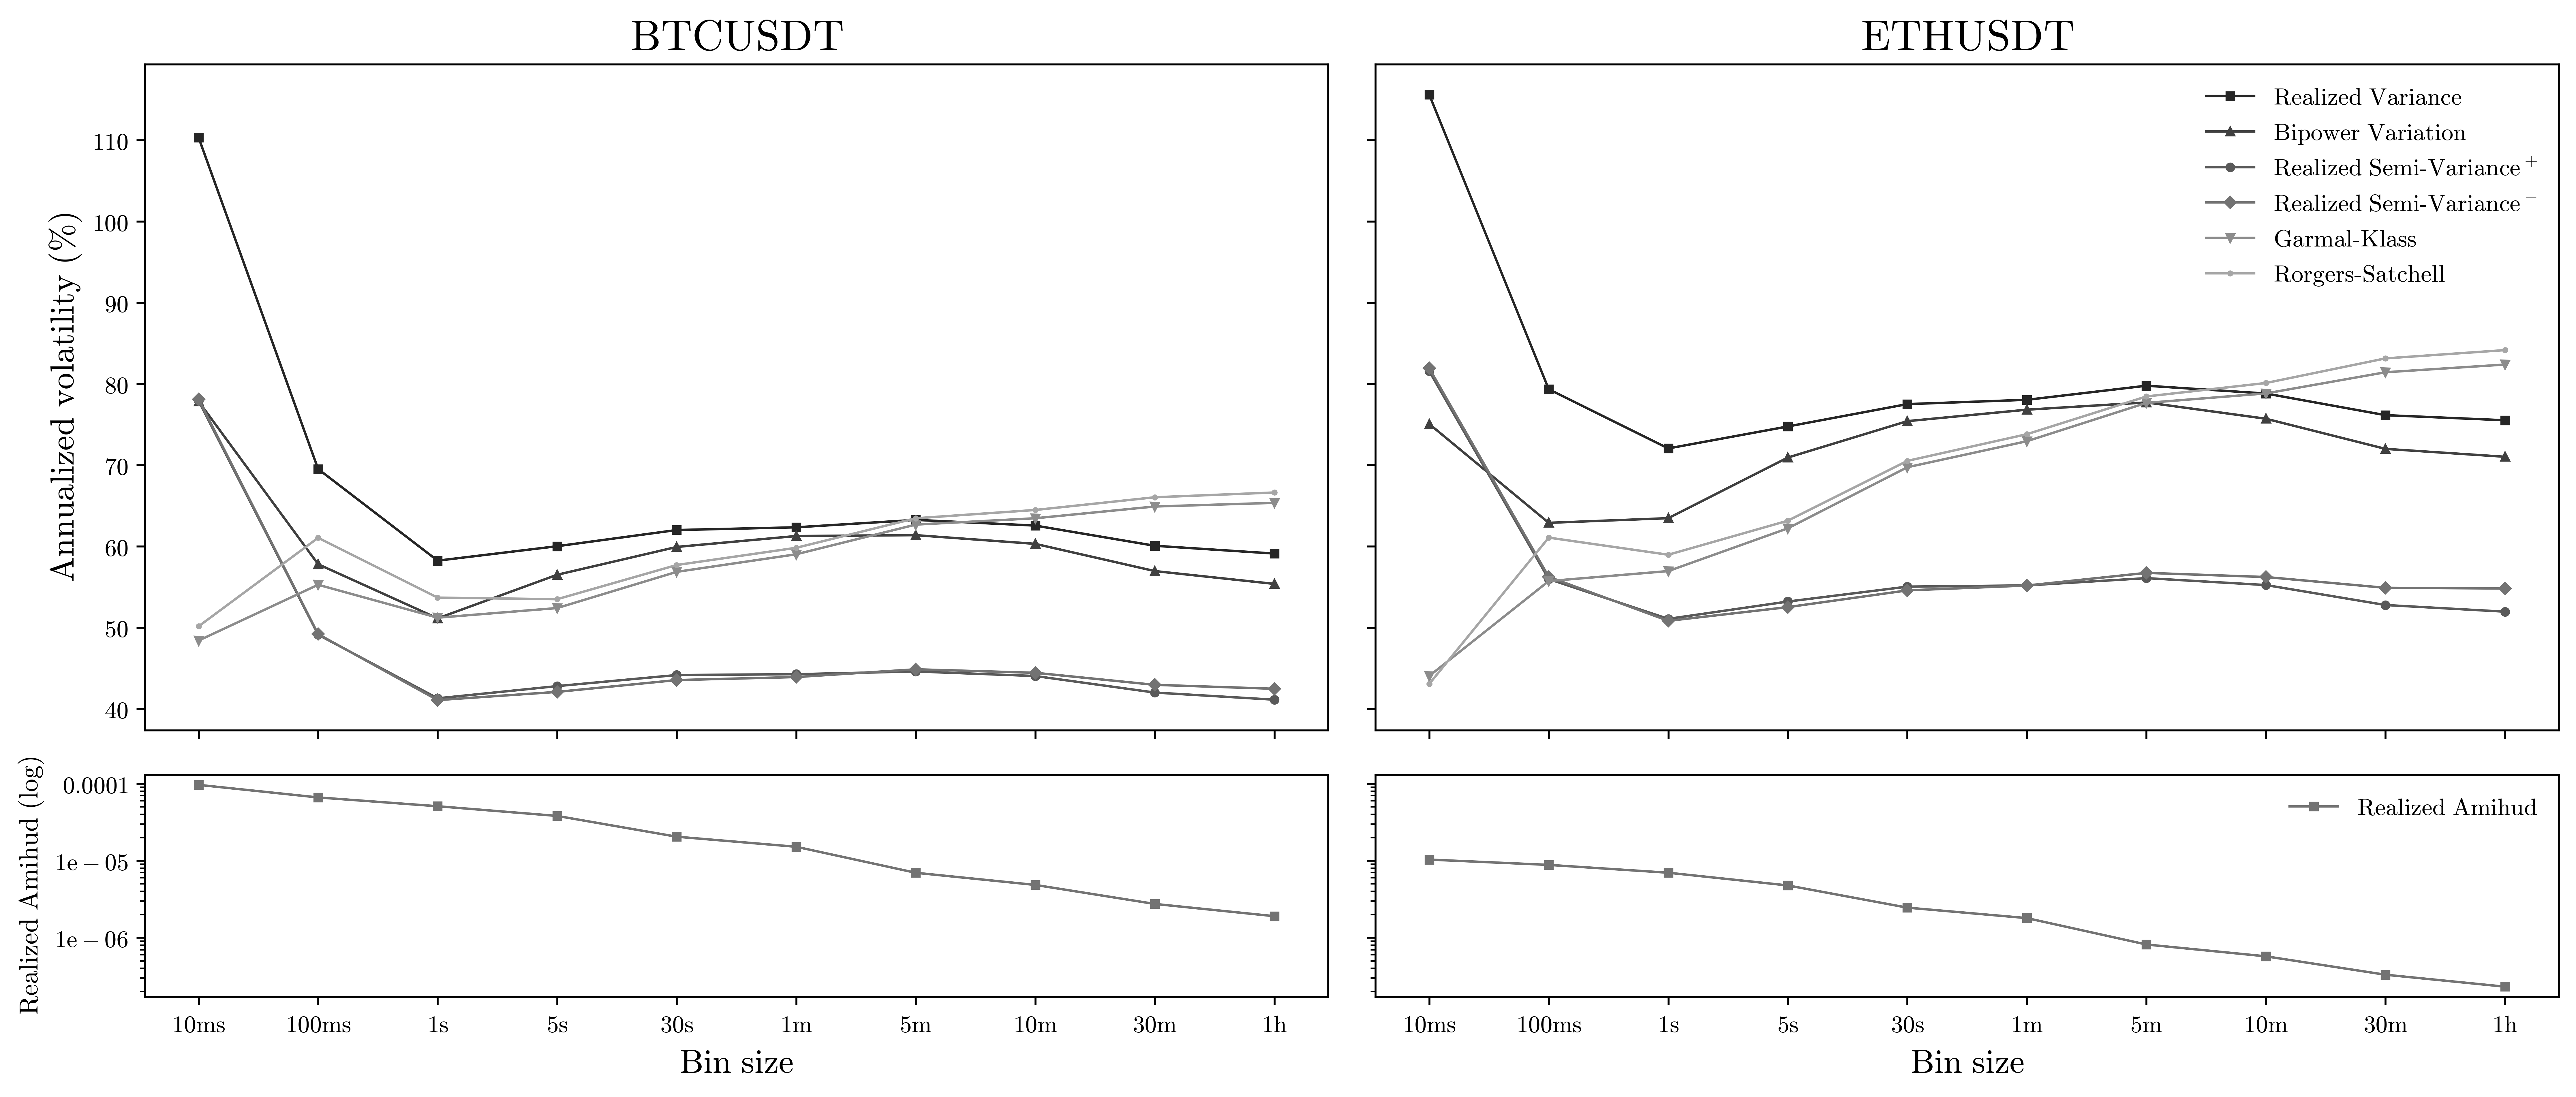
\includegraphics[width=1\textwidth]{media/signaturePlot.png}
\end{figure}



\section{Analysis and Hypothesis Testing}

\subsection{Events and Market Periods}

Using our 5m data, we begin by ploting daily price and dollar volume of both Ethereum and Bitcoin pairs, alongside all events explaining major volume spikes. We also add Binance's fee regime changes and Merge related announcements to the chart. Figure ~\ref{fig:events} underlines a factor 2 difference in volume (mean ETH daily volume is \$1.2B while it is \$2.7B for BTC) over the large difference in price between these two assets. From a purely visual perspective, Merge announcements (13, 14) are linked to little volume change, and Merge execution (16) is linked to a small-scale volume spike for Ethereum. However, event 16 has no observable effect for Bitcoin, on the contrary of the volume impact of event 15 (US inflation announcement higher than forecasted) for example. For Bitcoin, events 12 and 21, respectively Binance's removal then reintroduction of fees on Bitcoin pairs, are directly linked to a phase of sustained increased volume as trading becomes frictionless. For Bitcoin, mean volume increases 160\% compared to trading volume on the overall fee-present sample, while such effect is not to be observed for Ethereum, with a mean -26.4\% decrease during the fee-less phase. \medskip

Figure ~\ref{fig:feeRegime} illustrates this volume shift as fees regime change. Phase 1 corresponds to normal trading fees; phase 2 begins when Binance removed fees on 13 Bitcoin pairs; phase 3 starts when this zero-fee promotion is withdrawn from all pairs except BTCTUSDT; phase 4 represents the full reintroduction of fees. BTCUSDT volume rises sharply during phase 2 and drops immediately once fees are reinstated, underlining how fee regime impacts market behavior. BTCTUSD shows a volume spike as well once it becomes the only fee-free Bitcoin pair listed on Binance. Coinbase volume analysis shows a stable trend throughout these periods, underlining how these volumes changes are linked to Binance promotional-stunt rather than global market context. It is omitted from the figure due to its different scale. (lister les fees avant, pendant et après, pour BTC et ETH) \medskip

\begin{figure}[!htbp]
\centering
\caption{Daily price and dollar volume of ETHUSDT and BTCUSDT with major market events}
\vspace{8pt}
\label{fig:events}
\includegraphics[width=1\textwidth]{media/events.png}
\end{figure}

\begin{figure}[!htbp]
\centering
\caption{Trading volume across Binance fee regime phases for BTCUSDT and BTCTUSD}
\vspace{8pt}
\label{fig:feeRegime}

\includegraphics[width=1\textwidth]{media/feeRegime.png}
\end{figure}


Plotting these context events allows us to define three defined market periods shared by both assets, indicated by the background's grey shade. Period 1 (405 days) follows the DeFi summer and is characterized by increased volatility as prices peak before plummeting as crypto exchanges go bankrupt. Period 2 (from event 11 to event 26, 577 days) is characterized by regulatory changes, as the market moves more horizontally. Finally, Bitcoin spot ETFs approval marks the beginning of period 3 (356 days), where institutional investors get to invest in a more choppy market influenced by the beginning of the Trump administration. Beyond these shared contextual periods (53\% of Bitcoin-relevant events also affect Ethereum, and 72\% of events hold in the opposite direction) and the visual impression of joint movement, we verify whether this apparent co-dependence holds statistically using cointegration tests. \medskip
 

\subsection{Cointegration testing}
Cointegration allows us to verify if two assets share a long-term equilibrium relation while individual prices remain non-stationary. We use Engle-Granger (\cite{Engle1987}) which regresses one price serie on the other and tests the residual for stationarity via an Augmented Dickey-Fuller test: 

\begin{align}
y_t &= \alpha + \beta x_t + u_t \tag{9}\\
\Delta \hat u_t &= \rho \hat u_{t-1} + \sum_{i=1}^k \phi_i \Delta \hat u_{t-i} + \varepsilon_t \tag{10}
\end{align}

with $H_0:\rho=0$ (no cointegration). This approach depends on which variable is chosen as a regressor and only handles a single cointegration relation, we hence complement it using the Johansen trace test (\cite{Johansen1988}), based on a vector error-correction representation, which is symmetric by construction:

\begin{align}
\Delta Y_t &= \Pi Y_{t-1} + \sum_{i=1}^{k-1}\Gamma_i \Delta Y_{t-i} + \varepsilon_t \tag{11}
\end{align}

where $\Pi=\alpha\beta '$ and rank $(\Pi)=r$ gives the number of cointegrating vectors, tested via

\begin{align}
\lambda_{trace}(r) = -T\sum_{i=r+1}^{n}\ln(1-\hat\lambda_i) \tag{12}
\end{align}

with $\hat{\lambda_i}$ the ordered eigenvalues of $\Pi$. \medskip

According to both test, the full sample presents no significant cointegration (table~\ref{tab:cointegration}) despite a 0.81 price correlation, indicating that long-term correlated movements are destabilized by asymmetric shocks. This observation is evidenced in our event plots (figure~\ref{fig:events}): despite over half of news being shared by both pairs, many events impacting Ethereum are missing from the Bitcoin plot, and the opposite holds true. As for subperiods, the first one shows significant cointegration according to Engle-Granger (5\%) and both Johansen rank 0 (1\%) and rank 1 (5\%) tests, also highlighted by a 94\% correlation indicating non-stationary prices moving together. Cointegration weakens but remains present over period 2, emphasized by significant Engle-Granger (5\%) and Johansen rank 0 (10\%) tests. Period 3 presents no cointegration and a 0.62 correlation. This appears to be coherent with the "Bitcoin decoupling" hypothesis that can be drawn from events of this period. The arrival of crypto-ETFs as early as January of 2024 for Bitcoin and only six months later -- in July of 2024 -- for Ethereum might have led to a a temporary mismatch in investment vehicles for financial institutions between the two assets, leading to diverging market behavior.

\begin{table}[!htbp]
\centering
\small
\caption{Engle-Granger and Johansen cointegration test results, ETHUSDT-BTCUSDT, by period}
\vspace{4pt}
\label{tab:cointegration}
\renewcommand{\arraystretch}{1.3}
\begin{tabular}{lllll}
\textbf{Period}   & \textbf{Engle-Granger} & \textbf{Johansen (r$\le$0)}  & \textbf{Johansen (r$\le$1)}  & \textbf{Correlation} \\
\hline
Global  & Not significant                         & Not significant & Not significant & 0.81        \\
Period 1 & **                                      & ***             & **              & 0.94        \\
Period 2 & **                                      & *               & Not significant & 0.90        \\
Period 3 & Not significant                         & Not significant & Not significant & 0.62  \\
\hline      
\end{tabular}
\end{table}


\subsection{Flight of capital from PoW to PoS}

We hypothetize that the Merge might have initiated or be preceded by a flight of capital from networks that underwent the PoW-to-PoS transition towards networks that remained PoW throughout this period. Ethereum falls in the former category while Bitcoin fits the latter, yet we also download Binance data for this period's top cryptocurrencies (BNB, XRP, DOGE, ADA, MATIC, DOT, LTC, SOL, SHIB, TRX, UNI, AVAX, BUSD). We obtain historical weekly market capitalization from \href{https://coinmarketcap.com/historical/}{CoinMarketCap's Cryptocurrency Historical Data Snapshot}, fro 2022-07-03 to 2022-11-27 in order to cover the entierty of the Merge period: before \href{https://blog.ethereum.org/2022/08/12/finalized-no-36}{the first Merge announcement} on 2022-08-12, throughout, and after the Merge (2022-09-15). We use consensus mechanism evolution for these coins, as of November 27, 2022, obtained through \textcite{AmoussouGuenou2024} supplementary appendix. \medskip

An initial visual study of volume and price for coins of varying consensus mechanism indicates no significant shift around the Merge period. Using a slope chart of market capitalization, we check for any relation between market capitalization and consensus mechanism throughout the Merge. Contrary to our hypothesis, no common trends are observed for coins that remained either PoW or PoS, nor for those that underwent the PoW-to-PoS transition during this eriod. Coins seemingly all move together from one week to another independent of consensus mechanism, prompting us not to explore the dynamics of other coins any further.
\subsection{HAR-RV Model}

To explore the dynamics linking volatility to volume, fees and liquidity, we use the Heterogeneous Autoregressive model of Realized Volatility (HAR-RV) introduced by \textcite{Corsi2009} to study how these variables affect models' performances. HAR-RV is a three factor stochastic volatility model with a simple autoregressive structure enabling treatment of cascading volatilities realized over intervals of respectively one day, one week and one month. According to \textcite{Andersen2007}, it has shown remarkably good forecasting performance comparable to more complicated long-memory ARMIA model, as its varying horizons represent fluctuating expectations over different timeframes for next period's volatility. Realized volatility over a $x$ trading days period is defined as the average of daily quantities

\begin{align}
RV_t^{(x)}&=\frac{1}{x}\left( RV^{(d)}_t + RV^{(d)}_{t-1d} + ... +  RV^{(d)}_{t-x-1d} \right) \tag{13}
\end{align}

where RV is the realized variance -- or realized volatility -- defined in Eq.~\ref{eq:rv}. The empirical HAR-RV model is specified as follows:

\begin{align}
RV_{t+1}&=c+\beta^{(d)}RV_t^{(1)}+\beta^{(w)}RV_t^{(5)}+\beta^{(m)}RV_t^{(20)}+e_{t+1d} \tag{14} \label{eq:HAR-RV}
\end{align}

A benefit of having such a simple model is that it can easily be extended by adding additional regressors, such as lagged trading volume. \textcite{Tseng2015} introduced volume in the model, following the intuition of \textcite{Clark1973} who states that both traded volume and volatility are driven by the same underlying "news" variable and will therefore be positively correlated. This relationship has been widely documented for stock markets, for instance by \textcite{Gallant1992} and \textcite{Andersen1996}. We also extend the model using illiquidity metrics, cross-asset volatility and Binance's fees regime in order to observe how these features impact model's performance.  \medskip


\subsubsection{Adaptation to crypto market 24/7 trading and bin choice}
Unlike the 252 trading days observed on traditional financial markets, crypto trading happens live around the clock, with no week-end or holidays break. This characteristic prompts us to consider an adapted version of the HAR-RV model: instead of defining Eq. 13 over a week of five trading days and a month of twenty, we consider the case of 24/7 markets for which a week consists of seven days and a month of thirty. \medskip

Figure ~\ref{fig:volume} shows shows that there is an apparent intra-day and weekly cycle of trading volume on Bitcoin and Ethereum pairs: midday have a higher volatiliy, while week-ends show limited volume. We hence prefer a classical 1-5-20 model over of 1-7-30 model: it appears that major crypto currencies volume follows classical investor attention span. Similar trends are observed for Coinbase data.

\begin{figure}[!htbp]
\centering
\caption{Intraday and weekly cycle of trading volume for ETHUSDT and BTCUSDT}
\vspace{8pt}
\label{fig:volume}
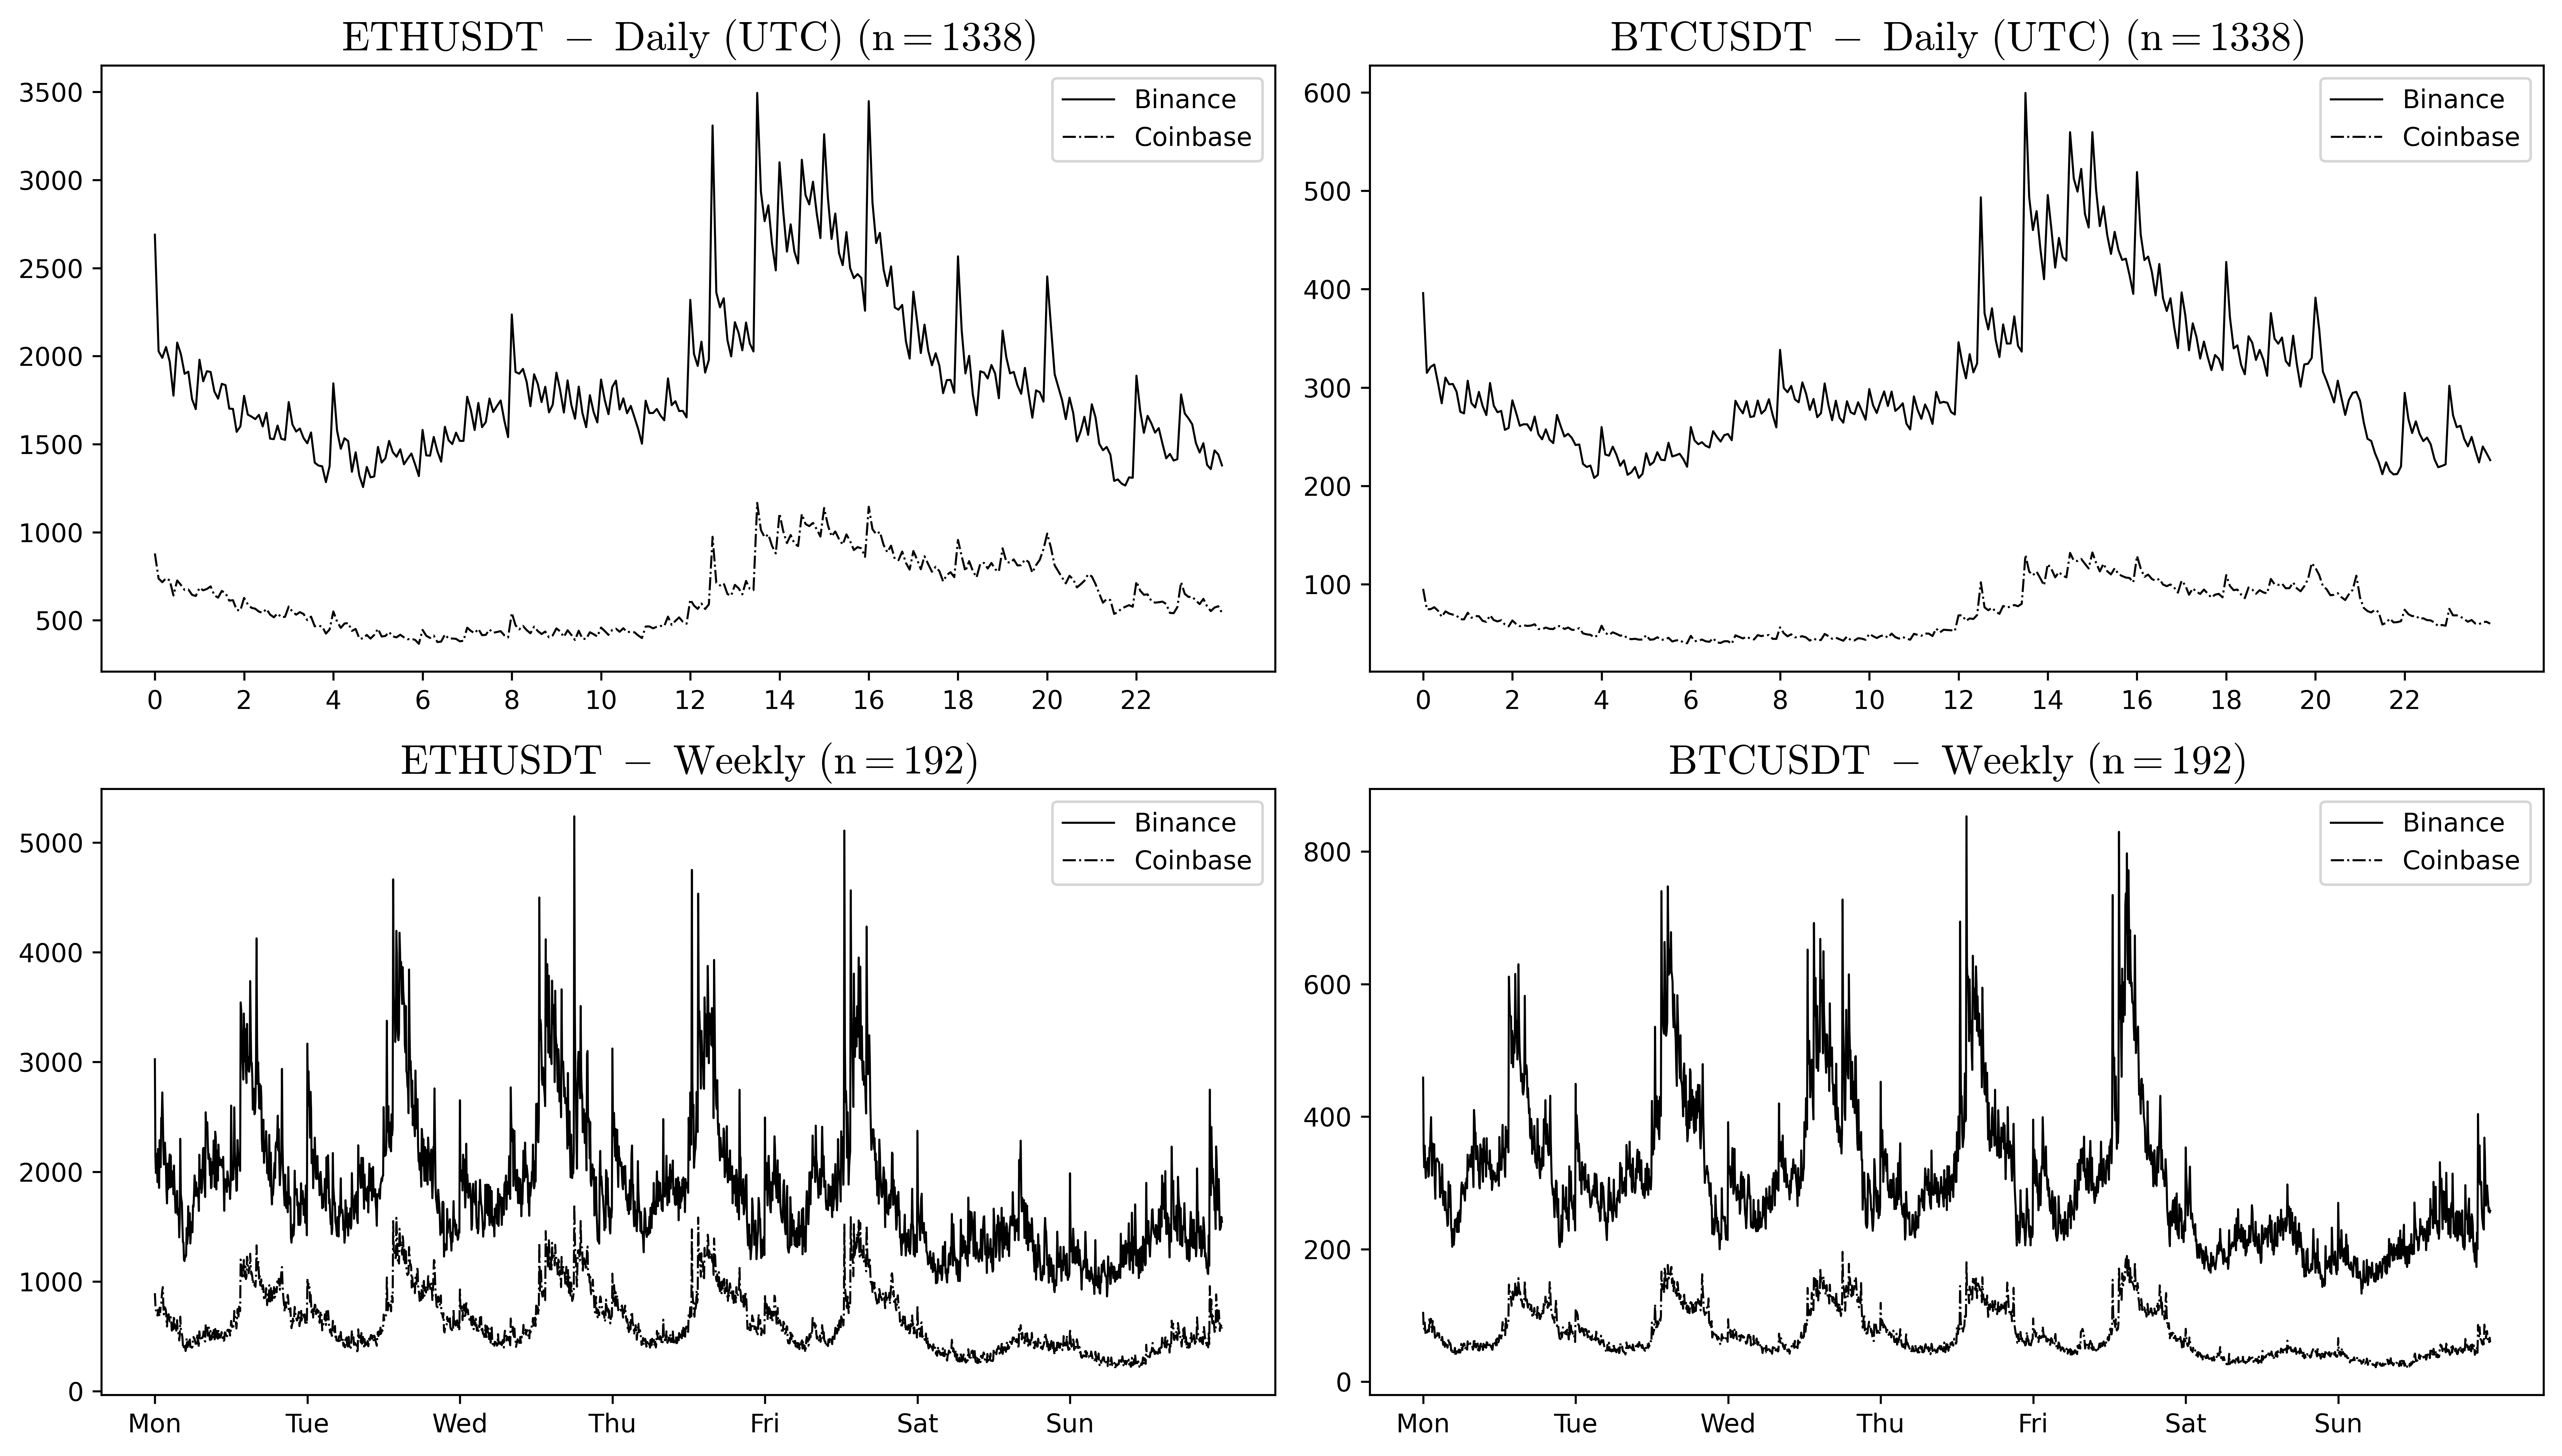
\includegraphics[width=1\textwidth]{media/volume.png}
\end{figure}

\subsubsection{Models}
Table ~\ref{tab:coefs} reports adjusted $R^2$ of features added individuallt to the base HAR-RV model, fitted over the full sample starting at the 21st day. The fee dummy variable equal 1 in the no-fee period, 0 otherwise. The jump component $jt$ follows \textcite{Andersen2007}, as

\begin{align}
jt_t(\Delta)= \max{(RV_t-BV_t, 0)} \tag{15} \label{eq:jump}
\end{align}

adding it to the base model reproduces their HAR-RV-J specification. Except for cross-asset volatility, jump component and dummy variables, features are added as three cascading regressors based on the 1 day, 5 days and 20 days average, following the different timeframes and horizons of the original model. \medskip

For Ethereum, only lagged volume and Kyle's $\lambda$ show meaningful individual improvement with individual adjusted $R^2$ of 0.2148 and 0.2025 respectively, compared to 0.1984 for the base model. Cross-asset volatility, the jump component and the fee dummy are not significant on their own. That is to be expected for the latter, as Ethereum doesn't undergo any fee regime change during the period tackled by the dummy variable. For Bitcoin, Kyle's lambda and the jump component brings the largest individual gains, with volume, Amihud's ratio, realized Amihud and the dummy offering moderate improvement. Notably, the dummy appears insignificant when considered individually, but becomes strongly significant (***) once combined with other regressors, suggesting its effects are conditional on controlling for volume, illiquidity and jumps. \medskip

\begin{table}[!htbp]
\centering
\small
\caption{Adjusted $R^2$ of HAR-RV model with individual added regressors, ETHUSDT \textit{\&} and BTCUSDT (n=1317)}
\vspace{4pt}
\label{tab:coefs}
\renewcommand{\arraystretch}{1.3}
\begin{tabular}{lllllllll}
\textbf{Adj. $R^{2}$} & \textbf{HAR-RV} & \textbf{Volume} & \textbf{Cross vol.} & \textbf{jt} & \textbf{Ami.} & \textbf{Rami.} & \textbf{Kyle's $\lambda$} & \textbf{Fees}  \\
\hline
ETH & 0.198     & 0.215         & 0.198           & 0.199     & 0.172          & 0.197          & 0.202                                     & 0.198 \\
BTC & 0.134     & 0.135         & 0.133           & 0.139     & 0.134          & 0.134          & 0.140                                     & 0.134 \\
\hline
\end{tabular}
\end{table}

Building on these results, we estimate additive models, summarized in table ~\ref{additive_full} for the entire sample and in Appendix~\ref{sec:appendixEvents} for sub-periods. For Ethereum over the full period, volume and Kyle's lambda substantially improve fit, jump component adds further improvement, but cross-volatility and fee-dummy marginally improve $R^2$ while deteriorating BIC. We retain the volume+Kyle+jump speficiation. Across sub-periods, features choice becomes seemingly regime dependent. Periode 1 and 3 show overall weak fit (adj. $R^2$ of 0.1318 and 0.0367 respectively) while penalizing complexity: the best model is the one driven by volume alone, while AIC and BIC suggest the base model would be preferred. Period 2 shows a much improved fit, with volume+Kyle+jump+cross-volatility reaching an 0.3971 adjusted $R^2$. This falls in line with our simple graphical analysis: period 1 and 3 show much higher volatility, while period 2 shows a stable price trend with fewer volume or volatility spikes. For Bitcoin over the full period, the specification volume+Kyle+jump component+cross-volatility+fee appears to have the best performance for both $R^2$ and AIC. The dummy's coefficient (-0.0007***) confirms its explanatory role once other factors are taken into account. Sub-period analysis shows a pattern quite similar to that of Ethereum: the volume+Kyle+jump model has the best performance for the first period, while period 2 favors the full specification with an increased fit (adj. $R^2$ of 0.2326), and period 3 shows negligbible explanatory power, with the base model being preferred by AIC and BIC. \medskip

Overall, past volatility and trading volume drive most of the explanatory power for both assets, as underlined by \textcite{Tseng2015}'s model. Microstructure metrics (Kyle's $\lambda$, jump component) add marginal improvement, while cross-asset volatility spillovers and fee-regime effects matter only conditionally. Period 2 outperformance for both pairs suggests that volatility dynamics are more predictable by our regression in low-volatility episodes rather than during volatile episodes.

\begin{table}[!htbp]
\centering
\small
\caption{Additive HAR-RV models estimates with additional regressors, full sample, ETHUSDT \textit{\&} BTCUSDT}
\vspace{4pt}
\label{tab:additive_full}
\renewcommand{\arraystretch}{1.3}
\begin{tabular}{l*{6}{c}}
\multicolumn{7}{l}{\textbf{A.} ETHUSDT (n=1317)} \\
& \textbf{base} & \textbf{+volume} & \textbf{+kyle} & \textbf{+jt} & \textbf{+cross\_vol} & \textbf{+fees} \\
\hline
const & \hfil 0.0007*** & \hfil -0.0087*** & \hfil -0.0106*** & \hfil -0.0107*** & \hfil -0.0108*** & \hfil -0.0121*** \\
$RV_1$ & \hfil 0.1802*** & \hfil 0.1312*** & \hfil 0.1545*** & \hfil 0.1829*** & \hfil 0.2421*** & \hfil 0.2534*** \\
$RV_5$ & \hfil 0.1668*** & \hfil 0.1609*** & \hfil 0.1680*** & \hfil 0.1554*** & \hfil 0.1507*** & \hfil 0.1521*** \\
$RV_{20}$ & \hfil 0.0965*** & \hfil 0.0341 & \hfil -0.0900** & \hfil -0.0889* & \hfil -0.0895* & \hfil -0.0975** \\
$vol_1$ & & \hfil 0.0003 & \hfil 0.0003* & \hfil 0.0003* & \hfil 0.0003* & \hfil 0.0003** \\
$vol_5$ & & \hfil 0.0002 & \hfil 0.0003 & \hfil 0.0004 & \hfil 0.0004 & \hfil 0.0004 \\
$vol_{20}$ & & \hfil 0.0003 & \hfil 0.0003 & \hfil 0.0002 & \hfil 0.0002 & \hfil 0.0003 \\
$kyle_1$ & & & \hfil -0.1295 & \hfil -0.1370 & \hfil -0.1296 & \hfil -0.1265 \\
$kyle_5$ & & & \hfil -0.3490* & \hfil -0.3434* & \hfil -0.3459* & \hfil -0.3584* \\
$kyle_{20}$ & & & \hfil 0.6610*** & \hfil 0.6543*** & \hfil 0.6604*** & \hfil 0.6381*** \\
$jt$ & & & & \hfil -0.2924 & \hfil -0.2862 & \hfil -0.2703 \\
cross\_vol & & & & & \hfil -0.1099 & \hfil -0.1381 \\
fees & & & & & & \hfil -0.0003* \\
\hline
$R^2$ & \hfil 0.2003 & \hfil 0.2184 & \hfil 0.2304 & \hfil 0.2318 & \hfil 0.2324 & \hfil 0.2343 \\
Adj. $R^2$ & \hfil 0.1984 & \hfil 0.2148 & \hfil 0.2251 & \hfil 0.2259 & \hfil 0.2259 & \hfil 0.2272 \\
AIC & \hfil -12829.73 & \hfil -12853.90 &   \hfil -12868.36 & \hfil -12868.64 & \hfil -12867.72 & \hfil -12868.92 \\
BIC & \hfil -12809.00 & \hfil -12817.62 & \hfil -12816.53 & \hfil -12811.62 & \hfil -12805.52 & \hfil -12801.54 \\
\hline
\\[2pt]
\multicolumn{7}{l}{\textbf{B.} BTCUSDT (n=1317)} \\
& \textbf{base} & \textbf{+volume} & \textbf{+kyle} & \textbf{+jt} & \textbf{+cross\_vol} & \textbf{+fees} \\
\hline
const & \hfil 0.0005*** & \hfil 0.0005 & \hfil 0.0004 & \hfil 0.0003 & \hfil 0.0003 & \hfil -0.0031*** \\
$RV_1$ & \hfil 0.1482*** & \hfil 0.1383*** & \hfil 0.1652*** & \hfil 0.2224*** & \hfil 0.2293*** & \hfil 0.1331 \\
$RV_5$ & \hfil 0.1386*** & \hfil 0.0941* & \hfil 0.0708 & \hfil 0.0485 & \hfil 0.0494 & \hfil 0.0198 \\
$RV_{20}$ & \hfil 0.1319*** & \hfil 0.1746*** & \hfil 0.1110** & \hfil 0.1190*** & \hfil 0.1190*** & \hfil 0.0746 \\
$vol_1$ & & \hfil 0.0000 & \hfil 0.0000 & \hfil 0.0000 & \hfil 0.0000 & \hfil 0.0001 \\
$vol_5$ & & \hfil 0.0003* & \hfil 0.0004** & \hfil 0.0004** & \hfil 0.0004** & \hfil 0.0006*** \\
$vol_{20}$ & & \hfil -0.0004** & \hfil -0.0005*** & \hfil -0.0005*** & \hfil -0.0005*** & \hfil -0.0004** \\
$kyle_1$ & & & \hfil -0.0006* & \hfil -0.0007* & \hfil -0.0007* & \hfil -0.0006 \\
$kyle_5$ & & & \hfil -0.0001 & \hfil 0.0000 & \hfil 0.0000 & \hfil -0.0001 \\
$kyle_{20}$ & & & \hfil 0.0015** & \hfil 0.0014** & \hfil 0.0015** & \hfil 0.0014** \\
$jt$ & & & & \hfil -0.5365*** & \hfil -0.5411*** & \hfil -0.4813*** \\
cross\_vol & & & & & \hfil -0.0042 & \hfil 0.0408 \\
fees & & & & & & \hfil -0.0007*** \\
\hline
$R^2$ & \hfil 0.1356 & \hfil 0.1394 & \hfil 0.1494 & \hfil 0.1552 & \hfil 0.1552 & \hfil 0.1637 \\
Adj. $R^2$ & \hfil 0.1336 & \hfil 0.1354 & \hfil 0.1435 & \hfil 0.1487 & \hfil 0.1480 & \hfil 0.1560 \\
AIC & \hfil -14083.88 & \hfil -14083.61 & \hfil -14093.08 & \hfil -14100.02 & \hfil -14098.03 & \hfil -14109.40 \\
BIC & \hfil -14063.15 & \hfil -14047.33 & \hfil -14041.25 & \hfil -14043.01 & \hfil -14035.83 & \hfil -14042.02 \\
\hline
\end{tabular}
\begin{tablenotes}
\small
\item * $p<.1$, ** $p<.05$, *** $p<.01$
\end{tablenotes}
\end{table}

\subsubsection{Forecasting: volatility proxy and loss functions}

The evaluation of volatility foreacst is hindered by the fact that the variable of interest -- conditional variance -- is never directly observed. \textcite{Patton2011} shows that choice of proxy matters in this case, as certain loss functions can lead to distorted ranking of competing forecasts. He derives conditions for a loss function to be "robust" to such distortion and shows that only mean squared-error (MSE, Eq.~\ref{eq:MSE}) and QLIKE (~\ref{eq:QLIKE}) loss functions satisfy them. MSE penalizes the squared forecast error symmetrically, while QLIKE penalizes the standardized error, making it less sensitive to the scale of volatility itself.

\begin{align}
    L_{MSE}(\hat{\sigma}^2,h)&=(\hat{\sigma}^2-h) \tag{16} \label{eq:MSE}\\
    L_{QLIKE}(\hat{\sigma}^2,h)&=\log h+\frac{\hat{\sigma}^2}{h} \tag{17} \label{eq:QLIKE}
\end{align}

Between those candidates, we selecte QLIKE over MSE for two reasons presented by \textcite{Patton2011}. First, \textcite{Patton2009} shows that Diebold-Mariano-West tests of equal predictive accuracy -- which test whether one forecast is significantly more accurate than another, on average --  have higher power using QLIKE loss than under MSE loss. Second, since QLIKE uses standardized error $\hat{\sigma}^2 / h$ rather than raw error $\hat{\sigma}^2-h$, it is lense sensible to extreme observations, which is relevant in our case since heterogenous volatility regimes are observed depending on period. It is hence why results are presented using QLIKE loss over MSE loss. As for volatility proxy, we retain realized volatility (Eq. ~\ref{eq:rv}) rather than other volatility proxies such as bipower variation (Eq. ~\ref{eq:bv}) for the following reason. In our setting, the jump component (Eq. ~\ref{eq:jump}) implies that BV would be a biased proxy whenever jumps are present, and would hence violate the assumption A1 required for Patton's robustness result. Moreover, all specifications are trained to predict $RV_{t+1}$ along standard HAR-RV recommandations (\cite{Corsi2009}), so RV is the natural proxy for out-of-sample evaluation: employing BV would introduce a mismatch between estimation and evaluation targets that could differ in scale. \medskip

For each specification, we compute one-step-ahead out-of-sample forecasts of $RV_{t+1}$. We use an expanding window to estimate our coefficients: starting from an initial training window covering 80\% of the relevant period chronological observations, the model is re-estimated at each step $t$ using all data available up to $t$ in order to forecast $RV_{t+1}$. Window is then extended by one observation and the procedure is repeated through the end of the period for the remaining 20\% of out-of-sample data. We then compute the QLIKE loss function for each forecast and report the average over the entire period. We experiment with individual variables added to the base HAR-RV model, as well as additive models that aren't shown here as they didn't have the highest out-of-sample performance. We also experiment with models regressing volume and Kyle's lambda alone on realized volatility, without the base HAR-RV component, altough we follow the cascading structure over 1, 5 and 20 days averages of Eq.~\ref{eq:HAR-RV}. Results are showcased in table ~\ref{tab:forecast}. \medskip

\begin{table}
\centering
\small
\caption{Out-of-sample QLIKE forecast losses by model and sub-period, ETHUSDT \textit{\&} BTCUSDT}
\vspace{4pt}
\label{tab:forecast}
\renewcommand{\arraystretch}{1.3}
\setlength{\tabcolsep}{10pt}
\begin{tabular}{lcccc}
\multicolumn{5}{l}{\textbf{A.} ETHUSDT} \\
& \multicolumn{4}{c}{\textbf{Period}} \\
\cline{2-5}
\textbf{Model} & \textit{Full}    & \textit{1}          & \textit{2}          & \textit{3} \\
\hline
HAR-RV      & \textbf{-5.7029}    & -5.0732             & -6.2430             & -5.4564 \\
+volume     & -5.5225             & \underline{-5.1888} & -6.0837             & \underline{-5.5136} \\
+Kyle       & -5.6794             & -5.0630             & -6.2390             & -5.4509 \\
+cross\_vol & -5.6991             & -5.0660             & -6.2323             & -5.4559 \\
+jt         & \underline{-5.7009} & -5.0921             & \underline{-6.2537} & -5.4644 \\
volume      & -5.4884             & \textbf{-5.2435}    & -6.0717             & \textbf{-5.5673} \\
Kyle        & -5.6850             & -4.9338             & \textbf{-6.2944}    & -5.3841 \\
\hline
\\[2pt]
\multicolumn{5}{l}{\textbf{B.} BTCUSDT} \\
& \multicolumn{4}{c}{\textbf{Period}} \\
\cline{2-5}
\textbf{Model} & \textit{Full}    & \textit{1}          & \textit{2}          & \textit{3} \\
\hline
HAR-RV      & -6.1551             & -5.5123             & \underline{-6.2215} & -6.0362 \\
+volume     & -6.1519             & \underline{-5.5743} & -6.0238             & -5.9833 \\
+Kyle       & -6.1226             & -5.4839             & -6.0784             & -6.0261 \\
+cross\_vol & -6.1519             & -5.5004             & -6.2105             & -6.0247 \\
+jt         & \underline{-6.1588} & -5.5193             & \textbf{-6.2299}    & \underline{-6.0386} \\
volume      & \textbf{-6.1670}     & \textbf{-5.6179}    & -6.0668             & \textbf{-6.0658} \\
Kyle        & -6.1353             & -5.3994             & -6.1518             & -6.0209 \\
\hline
\end{tabular}
\begin{tablenotes}
\small
\item Bold indicates the best model for the period, underlined indicates second best.
\end{tablenotes}
\end{table}


For Ethereum over the full period, base HAR-RV is the best model. All addition of individual variables worsen it, on the contrary to whats indicated in ~\ref{tab:additive_full}. For sub-periods, only volume and the jump component improve the model, with +volume+jump being the best model for period 1, +jump being the best model for period 2, and +volume being the best model for period 3. However, regressing volume itself on RV in a 1-5-20 fashion gives improved results compared to respective best models for period 1 and 3. For period 2, Kyle's lambda alone gives a higher QLIKE than HAR-RV+jump, suggesting that illiquidity proxy is a better indicator of volatility in periods of low volatility, as trade-level data carries more information than aggregated, small-scale, returns. \medskip

For Bitcoin, only the jump component improves the base model over the full period. For sub-periods, only volume and the jump component once again improve HAR-RV, with the best model being HAR-RV+volume for period 1 and HAR-RV+jump for period 2 and 3. Regressing volume alone still yields even higher results for period 1 and 3, while Kyle's lambda alone worsens performance for period 2. It is surprising that regressing volume alone yields better results than, for example, adding volume to the base volume. For exemple, in period 3, HAR-RV gives a QLIKE of -6.0362, while HAR-RV+volume gives -5.9833, and volume alone gives -6.0658. \medskip

Kyle's lambda as a predictor of volatilty alone in period 2 of ETH isn't enough, as it isn't matched by period 2 of BTC. However, volume alone stronger performance in period 1 and 3 for both assets underline enhanced prediction power for periods of higher volatility. \medskip

\appendix
\section{Events Timeline}
\label{sec:appendixEvents}

List of events linked to main volume spikes for Ethereum and Bitcoin USDT pairs on Binance, from 2021-05 to 2024-12.

\begin{description}
    \item[2021] \hfill \\ 1. 2021-05-19 -- Major crypto market crash amplified by high leverage and cascading liquidations \\ 2. 2021-06-22 -- China steps up efforts against Bitcoin \\ 3. 2021-07-26 -- Amazon's Bitcoin rumors skyrocket prices, liquidating \$1B in short BTC positions \\ 4. 2021-08-05 -- Ethereum network; London hard fork \\ 5. 2021-09-07 -- Bitcoin becomes legal currency in El Salvador \\ 6. 2021-12-04 -- Spot selling drives price drop, triggering a long squeeze in the derivatives market 

    \item[2022] \hfill \\ 7. 2022-01-21 -- Anticipation of Fed rates hike \\ 8. 2022-02-24 -- Market-wide selloff following Ukraine invasion \\ 9. 2022-05-09 -- Beginning of the LUNA/UST depeg and Terra collapse \\ 10. 2022-05-12 -- LUNA/UST depeg, Terra ecosystem collapse \\ 11. 2022-06-13 -- Celsius blocks customer withdrawals \\ 12. 2022-07-08 -- Binance launches zero fee bitcoin trading \\ 13. 2022-08-12 -- Ethereum network; Mainnet Merge incoming (blog announcement) \\ 14. 2022-08-24 -- Ethereum network; Mainnet Merge Announcement (official announcement) \\ 15. 2022-09-13 -- US inflation higher than expected, reinforcing fear of Fed rates hike \\ 16. 2022-09-15 -- Ethereum network; Paris upgrade (the Merge) \\ 17. 2022-09-27 -- Bank of England stabilizing UK bond market fuels hopes of eased rates hike \\ 18. 2022-11-08 -- FTX halts withdrawals, Binance announces then cancels FTX acquisition 

    \item [2023] \hfill \\ 19. 2023-01-12 -- US slowing inflation drives prices up \\ 20. 2023-03-14 -- Fed protecting SVB and Signature Bank deposits eases banking contagion fears \\ 21. 2023-03-22 -- Binance stops zero fee bitcoin trading \\ 22. 2023-06-21 -- BlackRocks's Bitcoin ETF sparks institutional buying \\ 23. 2023-08-17 -- Crypto sinks on rising US bond yields \\ 24. 2023-10-24 -- Growing anticipation of imminent BlackRock spot ETF approval \\ 25. 2023-11-09 -- Rally fueled by anticipation of spot Bitcoin ETF approval
    
    \item [2024] \hfill \\ 26. 2024-01-10 -- SEC approves first US spot Bitcoin ETFs \\ 27. 2024-01-10 -- Inflows into new spot Bitcoin ETFs outpace Bitcoin supply \\ 28. 2024-03-05 -- Bitcoin reaches ATH, followed by profit-taking \\ 29. 2024-03-20 -- Rates are maintained but rate cuts are projected \\ 30. 2024-04-13 -- Iranian drone attack on Israel \\ 31. 2024-05-23 -- SEC approves filing for spot Ethereum ETFs \\ 32. 2024-07-05 -- Mt. Gox exchange starts repaying \$9B in Bitcoin to creditors \\ 33. 2024-08-05 -- Unwinding of the yen carry trade: VIX spike, Ethereum sales by Jump Trading \\ 34. 2024-11-06 -- Trump's election sparks a crypto rally \\ 35. 2024-11-11 -- Market rally pricing friendlier Trump administration after elections win \\ 36. 2024-12-05 -- Bitcoin crosses \$100,00 after Trump names Paul Atkin as next SEC chair
    
\end{description} 

\section{Correlation Analysis}
\label{sec:appendixHeatmap}

\begin{figure}[!htbp]
\centering
\caption{Correlation heatmap of volatility and liquidity metrics across intraday frequencies}
\vspace{8pt}
\label{fig:AppendixHeatmap}
\includegraphics[width=1\textwidth]{media/correlationHeatmap.png}
\end{figure}

Daily metrics correlation are measured over 1338 days, with each day's estimate built from multiple intraday bin sizes (10ms, 1s and 5m). \medskip

Across both assets, realized and range-based volatility estimators converge at 10ms then split into trade-based and range-based families capturing distinct volatility components at 1s, before reconverging at 5m. This behavior is consistent with high frequency microstructure noise imposing a common variance structure independent of estimator type (\cite{Hansen2006}; \cite{Bandi2008}). Once this noise disapears, a mild upside/downside asymmetry is observed for BTCUSDT only. Volatility and liquidity correlation flips as scale increases, from Realized Amihud at 10ms bins to Kyle's lambda at 5m bins, while Amihud remains uncorrelated. Relationship with price is nonexistant at every scale, and link to volume peaks at 1s. \medskip

Liquidity measures show a similar granularity dependence depending on asset. For BTCUSDT, correlation between Amihud and Realized Amihud strengthens as bin size increases and more trades are aggregated within each bin. Correlation of Amihud remains negative for all illiquidity measures for ETHUSDT. For both assets, Kyle's lambda moves closer to realized Amihud as bin size reduces, suggesting price impact and realized illiquidity reflect the same phenomenon at the trade level but diverge over longer intervals. As expected, Amihud and Kyle's lambda have a stabel relationship with price and volume (both are computed independently of bin size), while Realized Amihud becomes negatively correlated with volume as bin size increases. \medskip

\section{Additive Models by Sub-period}
\label{sec:appendixSubperiods}

\begin{small}
\renewcommand{\arraystretch}{1.3}
\begin{longtable}{l*{6}{c}}
\caption{\parbox{\textwidth}{Additive HAR-RV models by sub-period, ETHUSDT \textit{\&} BTCUSDT}}\\
\label{tab:additive_subperiods}\\
\Needspace{15\baselineskip}
\multicolumn{7}{l}{\textbf{A.} ETHUSDT, Period 1 (n=386)} \\
& \textbf{base} & \textbf{+volume} & \textbf{+kyle} & \textbf{+jt} & \textbf{+cross\_vol} & \textbf{+fees} \\
\hline
const & \hfil 0.0013*** & \hfil -0.0088 & \hfil -0.0095 & \hfil -0.0093 & \hfil -0.0096 & \hfil -0.0096 \\
$RV_1$ & \hfil 0.0900 & \hfil 0.0146 & \hfil 0.0405 & \hfil 0.0379 & \hfil 0.0536 & \hfil 0.0536 \\
$RV_5$ & \hfil 0.1860*** & \hfil 0.1834** & \hfil 0.2068** & \hfil 0.2085** & \hfil 0.2071** & \hfil 0.2071** \\
$RV_{20}$ & \hfil 0.0517 & \hfil 0.0369 & \hfil -0.0402 & \hfil -0.0409 & \hfil -0.0423 & \hfil -0.0423 \\
$vol_1$ & & \hfil 0.0008 & \hfil 0.0007 & \hfil 0.0007 & \hfil 0.0007 & \hfil 0.0007 \\
$vol_5$ & & \hfil 0.0005 & \hfil 0.0005 & \hfil 0.0005 & \hfil 0.0005 & \hfil 0.0005 \\
$vol_{20}$ & & \hfil -0.0005 & \hfil -0.0004 & \hfil -0.0004 & \hfil -0.0004 & \hfil -0.0004 \\
$kyle_1$ & & & \hfil -0.0661 & \hfil -0.0630 & \hfil -0.0601 & \hfil -0.0601 \\
$kyle_5$ & & & \hfil -0.3840 & \hfil -0.3862 & \hfil -0.3884 & \hfil -0.3884 \\
$kyle_{20}$ & & & \hfil 0.4373 & \hfil 0.4372 & \hfil 0.4395 & \hfil 0.4395 \\
$jt$ & & & & \hfil 0.1935 & \hfil 0.1924 & \hfil 0.1924 \\
cross\_vol & & & & & \hfil -0.0293 & \hfil -0.0293 \\
fees & & & & & & \hfil 0.0000 \\
\hline
$R^2$ & \hfil 0.1318 & \hfil 0.1454 & \hfil 0.1500 & \hfil 0.1502 & \hfil 0.1502 & \hfil 0.1502 \\
Adj. $R^2$ & \hfil 0.1250 & \hfil 0.1318 & \hfil 0.1297 & \hfil 0.1275 & \hfil 0.1252 & \hfil 0.1252 \\
AIC & \hfil -3465.63 & \hfil -3465.73 & \hfil -3461.83 & \hfil -3459.91 & \hfil -3457.92 & \hfil -3457.92 \\
BIC & \hfil -3449.81 & \hfil -3438.04 & \hfil -3422.27 & \hfil -3416.39 & \hfil -3410.45 & \hfil -3410.45 \\
\hline
\\[2pt]
\Needspace{15\baselineskip}
\multicolumn{7}{l}{\textbf{B.} ETHUSDT, Period 2 (n=577)} \\
& \textbf{base} & \textbf{+volume} & \textbf{+kyle} & \textbf{+jt} & \textbf{+cross\_vol} & \textbf{+fees} \\
\hline
const & \hfil 0.0003*** & \hfil -0.0092*** & \hfil -0.0110*** & \hfil -0.0093*** & \hfil -0.0088*** & \hfil -0.0090*** \\
$RV_1$ & \hfil 0.3276*** & \hfil 0.3069*** & \hfil 0.2950*** & \hfil 0.4988*** & \hfil 0.6018*** & \hfil 0.6030*** \\
$RV_5$ & \hfil 0.1443** & \hfil 0.1463* & \hfil 0.2416*** & \hfil 0.1899** & \hfil 0.1877** & \hfil 0.1870** \\
$RV_{20}$ & \hfil 0.1421** & \hfil -0.1264 & \hfil -0.2589** & \hfil -0.2206** & \hfil -0.2072** & \hfil -0.2112** \\
$vol_1$ & & \hfil 0.0000 & \hfil 0.0000 & \hfil -0.0000 & \hfil 0.0000 & \hfil 0.0000 \\
$vol_5$ & & \hfil 0.0001 & \hfil 0.0002 & \hfil 0.0002 & \hfil 0.0002 & \hfil 0.0002 \\
$vol_{20}$ & & \hfil 0.0007** & \hfil 0.0008** & \hfil 0.0006* & \hfil 0.0005 & \hfil 0.0005 \\
$kyle_1$ & & & \hfil -0.1877 & \hfil -0.0182 & \hfil 0.0183 & \hfil 0.0190 \\
$kyle_5$ & & & \hfil -1.1307** & \hfil -1.1661*** & \hfil -1.1467*** & \hfil -1.1455*** \\
$kyle_{20}$ & & & \hfil 0.1568 & \hfil 0.1214 & \hfil 0.1429 & \hfil 0.1572 \\
$jt$ & & & & \hfil -1.1885*** & \hfil -1.1326*** & \hfil -1.1296*** \\
cross\_vol & & & & & \hfil -0.2164* & \hfil -0.2202* \\
fees & & & & & & \hfil -0.0000 \\
\hline
$R^2$ & \hfil 0.3339 & \hfil 0.3546 & \hfil 0.3745 & \hfil 0.4055 & \hfil 0.4086 & \hfil 0.4087 \\
Adj. $R^2$ & \hfil 0.3304 & \hfil 0.3478 & \hfil 0.3646 & \hfil 0.3950 & \hfil 0.3971 & \hfil 0.3961 \\
AIC & \hfil -5978.70 & \hfil -5990.87 & \hfil -6002.95 & \hfil -6030.33 & \hfil -6031.36 & \hfil -6029.40 \\
BIC & \hfil -5961.27 & \hfil -5960.36 & \hfil -5959.38 & \hfil -5982.39 & \hfil -5979.07 & \hfil -5972.75 \\
\hline
\\[2pt]
\Needspace{15\baselineskip}
\multicolumn{7}{l}{\textbf{C.} ETHUSDT, Period 3 (n=356)} \\
& \textbf{base} & \textbf{+volume} & \textbf{+kyle} & \textbf{+jt} & \textbf{+cross\_vol} & \textbf{+fees} \\
\hline
const & \hfil 0.0008*** & \hfil -0.0073** & \hfil -0.0069** & \hfil -0.0061* & \hfil -0.0062* & \hfil -0.0062* \\
$RV_1$ & \hfil 0.1043** & \hfil 0.0737 & \hfil 0.0646 & \hfil 0.1503 & \hfil 0.2230 & \hfil 0.2230 \\
$RV_5$ & \hfil 0.1274 & \hfil 0.1270 & \hfil 0.1140 & \hfil 0.1040 & \hfil 0.1028 & \hfil 0.1028 \\
$RV_{20}$ & \hfil -0.0002 & \hfil -0.2062 & \hfil -0.1544 & \hfil -0.1637 & \hfil -0.1646 & \hfil -0.1646 \\
$vol_1$ & & \hfil 0.0001 & \hfil 0.0001 & \hfil 0.0001 & \hfil 0.0001 & \hfil 0.0001 \\
$vol_5$ & & \hfil -0.0001 & \hfil -0.0001 & \hfil -0.0001 & \hfil -0.0001 & \hfil -0.0001 \\
$vol_{20}$ & & \hfil 0.0006 & \hfil 0.0006 & \hfil 0.0006 & \hfil 0.0006 & \hfil 0.0006 \\
$kyle_1$ & & & \hfil 0.0321 & \hfil 0.0453 & \hfil 0.0434 & \hfil 0.0434 \\
$kyle_5$ & & & \hfil 0.0811 & \hfil 0.0591 & \hfil 0.0626 & \hfil 0.0626 \\
$kyle_{20}$ & & & \hfil -0.1922 & \hfil -0.1833 & \hfil -0.1732 & \hfil -0.1732 \\
$jt$ & & & & \hfil -0.4091 & \hfil -0.4596 & \hfil -0.4596 \\
cross\_vol & & & & & \hfil -0.1139 & \hfil -0.1139 \\
fees & & & & & & \hfil 0.0000 \\
\hline
$R^2$ & \hfil 0.0356 & \hfil 0.0529 & \hfil 0.0544 & \hfil 0.0559 & \hfil 0.0568 & \hfil 0.0568 \\
Adj. $R^2$ & \hfil 0.0274 & \hfil 0.0367 & \hfil 0.0298 & \hfil 0.0285 & \hfil 0.0266 & \hfil 0.0266 \\
AIC & \hfil -3732.72 & \hfil -3733.16 & \hfil -3727.71 & \hfil -3726.28 & \hfil -3724.60 & \hfil -3724.60 \\
BIC & \hfil -3717.22 & \hfil -3706.04 & \hfil -3688.96 & \hfil -3683.66 & \hfil -3678.10 & \hfil -3678.10 \\
\hline
\\[2pt]
\Needspace{15\baselineskip}
\multicolumn{7}{l}{\textbf{D.} BTCUSDT, Period 1 (n=386)} \\
& \textbf{base} & \textbf{+volume} & \textbf{+kyle} & \textbf{+jt} & \textbf{+cross\_vol} & \textbf{+fees} \\
\hline
const & \hfil 0.0009*** & \hfil -0.0080* & \hfil -0.0093* & \hfil -0.0087* & \hfil -0.0084* & \hfil -0.0084* \\
$RV_1$ & \hfil 0.1036* & \hfil 0.0175 & \hfil 0.0483 & \hfil 0.0912 & \hfil 0.1178 & \hfil 0.1178 \\
$RV_5$ & \hfil 0.1016 & \hfil 0.0346 & \hfil 0.0392 & \hfil 0.0147 & \hfil 0.0202 & \hfil 0.0202 \\
$RV_{20}$ & \hfil 0.0812 & \hfil 0.0653 & \hfil 0.0019 & \hfil 0.0307 & \hfil 0.0335 & \hfil 0.0335 \\
$vol_1$ & & \hfil 0.0005 & \hfil 0.0004 & \hfil 0.0005 & \hfil 0.0005 & \hfil 0.0005 \\
$vol_5$ & & \hfil 0.0009 & \hfil 0.0011* & \hfil 0.0011* & \hfil 0.0011* & \hfil 0.0011* \\
$vol_{20}$ & & \hfil -0.0005 & \hfil -0.0006 & \hfil -0.0007 & \hfil -0.0007 & \hfil -0.0007 \\
$kyle_1$ & & & \hfil -0.0005 & \hfil -0.0004 & \hfil -0.0004 & \hfil -0.0004 \\
$kyle_5$ & & & \hfil -0.0013 & \hfil -0.0012 & \hfil -0.0012 & \hfil -0.0012 \\
$kyle_{20}$ & & & \hfil 0.0018 & \hfil 0.0016 & \hfil 0.0016 & \hfil 0.0016 \\
$jt$ & & & & \hfil -0.7365* & \hfil -0.7518* & \hfil -0.7518* \\
cross\_vol & & & & & \hfil -0.0162 & \hfil -0.0162 \\
fees & & & & & & \hfil 0.0000 \\
\hline
$R^2$ & \hfil 0.0707 & \hfil 0.0977 & \hfil 0.1056 & \hfil 0.1123 & \hfil 0.1124 & \hfil 0.1124 \\
Adj. $R^2$ & \hfil 0.0634 & \hfil 0.0834 & \hfil 0.0842 & \hfil 0.0886 & \hfil 0.0862 & \hfil 0.0862 \\
AIC & \hfil -3871.90 & \hfil -3877.31 & \hfil -3874.70 & \hfil -3875.58 & \hfil -3873.62 & \hfil -3873.62 \\
BIC & \hfil -3856.08 & \hfil -3849.62 & \hfil -3835.14 & \hfil -3832.07 & \hfil -3826.15 & \hfil -3826.15 \\
\hline
\\[2pt]
\Needspace{15\baselineskip}
\multicolumn{7}{l}{\textbf{E.} BTCUSDT, Period 2 (n=577)} \\
& \textbf{base} & \textbf{+volume} & \textbf{+kyle} & \textbf{+jt} & \textbf{+cross\_vol} & \textbf{+fees} \\
\hline
const & \hfil 0.0003*** & \hfil -0.0002 & \hfil 0.0000 & \hfil -0.0001 & \hfil 0.0000 & \hfil -0.0020 \\
$RV_1$ & \hfil 0.2113*** & \hfil 0.2131*** & \hfil 0.2158*** & \hfil 0.4049*** & \hfil 0.0643 & \hfil -0.0345 \\
$RV_5$ & \hfil 0.2311*** & \hfil 0.1649* & \hfil 0.1521* & \hfil 0.1120 & \hfil 0.1124 & \hfil 0.0704 \\
$RV_{20}$ & \hfil 0.0430 & \hfil 0.0837 & \hfil 0.0812 & \hfil 0.0770 & \hfil 0.0602 & \hfil 0.0239 \\
$vol_1$ & & \hfil -0.0000 & \hfil -0.0000 & \hfil -0.0000 & \hfil 0.0000 & \hfil 0.0000 \\
$vol_5$ & & \hfil 0.0003 & \hfil 0.0002 & \hfil 0.0002 & \hfil 0.0001 & \hfil 0.0003 \\
$vol_{20}$ & & \hfil -0.0002 & \hfil -0.0002 & \hfil -0.0002 & \hfil -0.0001 & \hfil -0.0001 \\
$kyle_1$ & & & \hfil -0.0000 & \hfil -0.0006 & \hfil 0.0001 & \hfil 0.0005 \\
$kyle_5$ & & & \hfil 0.0009 & \hfil 0.0011 & \hfil 0.0008 & \hfil 0.0011 \\
$kyle_{20}$ & & & \hfil -0.0004 & \hfil -0.0004 & \hfil -0.0011 & \hfil -0.0010 \\
$jt$ & & & & \hfil -0.9713*** & \hfil -0.7172*** & \hfil -0.5973*** \\
cross\_vol & & & & & \hfil 0.1866*** & \hfil 0.2255*** \\
fees & & & & & & \hfil -0.0005** \\
\hline
$R^2$ & \hfil 0.1905 & \hfil 0.1955 & \hfil 0.1963 & \hfil 0.2263 & \hfil 0.2433 & \hfil 0.2486 \\
Adj. $R^2$ & \hfil 0.1862 & \hfil 0.1870 & \hfil 0.1836 & \hfil 0.2127 & \hfil 0.2286 & \hfil 0.2326 \\
AIC & \hfil -6462.87 & \hfil -6460.48 & \hfil -6455.05 & \hfil -6475.03 & \hfil -6485.85 & \hfil -6487.88 \\
BIC & \hfil -6445.44 & \hfil -6429.97 & \hfil -6411.47 & \hfil -6427.09 & \hfil -6433.55 & \hfil -6431.23 \\
\hline
\\[2pt]
\Needspace{15\baselineskip}
\multicolumn{7}{l}{\textbf{F.} BTCUSDT, Period 3 (n=356)} \\
& \textbf{base} & \textbf{+volume} & \textbf{+kyle} & \textbf{+jt} & \textbf{+cross\_vol} & \textbf{+fees} \\
\hline
const & \hfil 0.0005*** & \hfil -0.0039* & \hfil -0.0031 & \hfil -0.0030 & \hfil -0.0029 & \hfil -0.0029 \\
$RV_1$ & \hfil 0.0653 & \hfil 0.0629 & \hfil 0.0990 & \hfil 0.0890 & \hfil 0.1544 & \hfil 0.1544 \\
$RV_5$ & \hfil 0.1871 & \hfil 0.2499 & \hfil 0.0909 & \hfil 0.1410 & \hfil 0.1436 & \hfil 0.1436 \\
$RV_{20}$ & \hfil 0.0752 & \hfil -0.2383 & \hfil -0.2587 & \hfil -0.2641 & \hfil -0.2668 & \hfil -0.2668 \\
$vol_1$ & & \hfil 0.0000 & \hfil 0.0000 & \hfil 0.0000 & \hfil 0.0000 & \hfil 0.0000 \\
$vol_5$ & & \hfil -0.0002 & \hfil -0.0002 & \hfil -0.0003 & \hfil -0.0003 & \hfil -0.0003 \\
$vol_{20}$ & & \hfil 0.0006 & \hfil 0.0006 & \hfil 0.0006 & \hfil 0.0006 & \hfil 0.0006 \\
$kyle_1$ & & & \hfil -0.0005 & \hfil -0.0003 & \hfil -0.0003 & \hfil -0.0003 \\
$kyle_5$ & & & \hfil 0.0020 & \hfil 0.0018 & \hfil 0.0018 & \hfil 0.0018 \\
$kyle_{20}$ & & & \hfil 0.0000 & \hfil 0.0001 & \hfil 0.0000 & \hfil 0.0000 \\
$jt$ & & & & \hfil -0.8196 & \hfil -0.8833 & \hfil -0.8833 \\
cross\_vol & & & & & \hfil -0.0378 & \hfil -0.0378 \\
fees & & & & & & \hfil 0.0000 \\
\hline
$R^2$ & \hfil 0.0322 & \hfil 0.0425 & \hfil 0.0515 & \hfil 0.0555 & \hfil 0.0559 & \hfil 0.0559 \\
Adj. $R^2$ & \hfil 0.0240 & \hfil 0.0260 & \hfil 0.0269 & \hfil 0.0281 & \hfil 0.0257 & \hfil 0.0257 \\
AIC & \hfil -3970.03 & \hfil -3967.82 & \hfil -3965.20 & \hfil -3964.69 & \hfil -3962.86 & \hfil -3962.86 \\
BIC & \hfil -3954.53 & \hfil -3940.69 & \hfil -3926.45 & \hfil -3922.07 & \hfil -3916.36 & \hfil -3916.36 \\
\hline
\multicolumn{7}{l}{\footnotesize * $p<.1$, ** $p<.05$, *** $p<.01$}
\end{longtable}
\end{small}


\setlength{\bibitemsep}{1em}
(le format des noms n'est pas partout le même)
\printbibliography

\end{setstretch}
\end{document}